\section{A survey of matrix mappings}
In the following pages we will look at three different kinds of mappings for a matrix $\Acc{m}{n}$: no frustration, frustration in one direction, frustration in both directions.

There are two different ways to view frustrated\index{frustration} mappings:
\begin{enumerate}
\item geometric deficiency\index{geometric deficiency} - mapping into a lower dimensional object;
\item algebraic deficiency\index{algebraic deficiency} - rank deficiency in row or column.
\end{enumerate}

In the examples that follow we will see ellipses mapped into other ellipses. These mappings are not frustrated. But once we map into a lower dimensional object, say from the unit sphere onto a line, the map is frustrated. This also means that we can't reverse the map. We can't make a finite linear map from a line with one parameter onto a sphere with three parameters.

These tables specify critical properties of the target matrix.

\textbf{Plots: }All plots start with the unit circle which is either
\begin{equation}
  \begin{array}{rcll}
     S(\theta) &=& \mat{c}{\cos \theta\\\sin \theta},\ \theta\in[0,2\pi) \qquad &n=2,\\
     S(\theta,\phi) &=& \mat{c}{\cos \theta\sin \phi\\\sin \theta \sin \phi\\\cos \phi},\ \theta\in[0,2\pi),\ \phi\in[0,\pi), \qquad &n=3.
  \end{array}
\end{equation}
Then look at the mapping action of the matrix. The result is either
\begin{equation}
  \A{}S(\theta) 
\end{equation}
when the target matrix has two columns or
\begin{equation}
  \A{}S(\theta,\phi) 
\end{equation}
when the target matrix has three columns.

The circles and ellipses have the color determined the the angular variable to provide an clearer idea of how the unit circle is distorted. So for the color red starts at $\theta=0$ and progresses through the spectrum until $\theta=2pi$ where the color is violet.\\

\textbf{Matrix images:} This block summarizes the plot above. For example, it may say that the plot represents a unit sphere being mapped to a line.\\

%%
\textbf{Vector space mappings:} These mappings are based on the dimensions of the spaces for the row and column vectors, $m$ and $n$. They disregard the issue of rank and and concerned purely with the mappings $\real{m}\mapsto\real{n}$ and  $\real{n}\mapsto\real{m}$. This map addresses the geometric deficiency of the mappings. For example are we going from a plane to a plane or a plane to a line. If the map is into a higher dimensional space we will have a frustrated map.\\

\textbf{Matrix ranks:} Are there rank deficiencies in the row or column space? If there is a rank deficiency we will see a frustrated map. 


\clearpage

%%
%% 2 x 2
%%
\begin{table}[htdp]
\begin{center}
\begin{tabular}{cc}
  $\A{}x=y$ & $\A{T}y=x$\\
 $\textellipsis$ & $\textellipsis$ \\
$\mat{rr}{1&2\\-1&2}\mat{c}{x_{1}\\x_{2}} = \mat{c}{y_{1}\\y_{2}}$ &
$\mat{rr}{1&-1\\2&2}\mat{c}{x_{1}\\x_{2}} = \mat{c}{y_{1}\\y_{2}}$ \\
\ \\
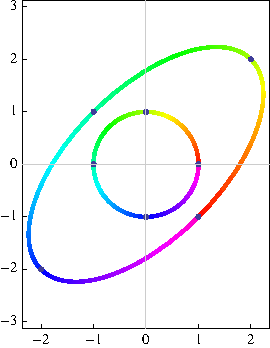
\includegraphics[ width = 2.15in ]{pdf/post_mortemII/2_2_2} &
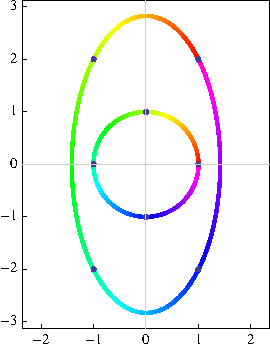
\includegraphics[ width = 2.15in ]{pdf/post_mortemII/2_2_2_t} \\
%%
\ \\
 matrix image & transpose matrix image \\
unit circle $\mapsto$ ellipse & unit circle $\mapsto$ ellipse\\
 $\textellipsis$ & $\textellipsis$ \\
vector space mappings & vector space mappings\\
(Domain) $\real{2} \mapsto \real{2}$ (Codomain) & (Codomain) $\real{2} \mapsto \real{2}$ (Domain)\\
 $\textellipsis$ & $\textellipsis$ \\
 full column rank  & full row rank\\
  $\textellipsis$ & $\textellipsis$ \\
 $\Ap=\AinvL$ & $\Ap=\AinvR$\\[10pt]
\end{tabular}
\end{center}
\label{tab:interpII:a}
\caption{Maps with no frustration. The domain and the codomain have the same dimension and the matrix has full rank. There are no null spaces associated with either the matrix or its transpose. The block dots are fiducial marks to help with comparing the orientation of the image (ellipse) relative to the target (circle). This matrix has full row rank, therefore the pseudoinverse is a left inverse. This matrix has full column rank, therefore the pseudoinverse is a right inverse. Because the pseudoinverse is both a left and a right inverse the pseudoinverse is also the standard inverse.}
\end{table}%

\clearpage
%%
%% 2 x 3
%%
\begin{table}[htdp]
\begin{center}
\begin{tabular}{cc}
  $\A{}x=y$ & $\A{T}y=x$\\
 $\textellipsis$ & $\textellipsis$ \\
$\mat{ccc}{0&3&0\\1&1&2}\mat{c}{x_{1}\\x_{2}\\x_{3}} = \mat{c}{y_{1}\\y_{2}}$ &
$\mat{cc}{0&1\\3&1\\0&2}\mat{c}{y_{1}\\y_{2}} = \mat{c}{x_{1}\\x_{2}\\x_{3}}$ \\
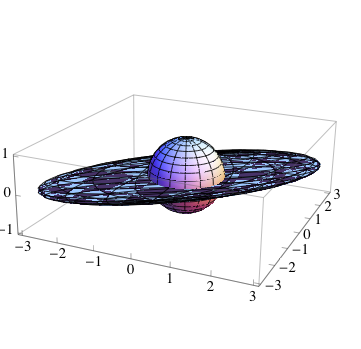
\includegraphics[ width = 2.5in ]{pdf/post_mortemII/3_2_2.png} &
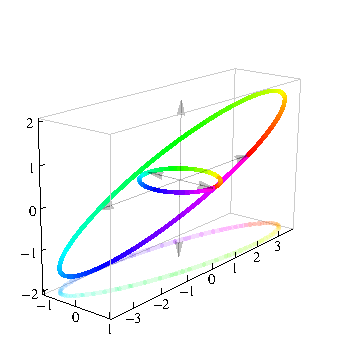
\includegraphics[ width = 2.5in ]{pdf/post_mortemII/3_2_2_t} \\
%%
vector space mappings & vector space mappings\\
(Domain) $\real{3} \mapsto \real{2}$ (Codomain) & (Codomain) $\real{2} \mapsto \real{3}$ (Domain)\\
 $\textellipsis$ & $\textellipsis$ \\
 matrix image & transpose matrix image \\
unit sphere $\mapsto$ elliptic disk & unit circle $\mapsto$ ellipse\\
 $\textellipsis$ & $\textellipsis$ \\
column rank deficient & full row rank\\
frustrated map\\
 $\textellipsis$ & $\textellipsis$ \\
 $\nexists\ \AinvL$ & $\Ap=\AinvR$\\[10pt]
\end{tabular}
\end{center}
\label{tab:interpII:a}
\caption{Frustration in one direction: domain to codomain. The frustration is signaled by the column rank deficiency where the matrix rank is less than the number of columns $(\rho<n)$. Notice that the mapping on the right is not frustrated; it is from a circle to an ellipse. Although both are two-dimensional objects, the ellipse is tipped and tilted out of the plane. The floor of the figure shows a shadow of the ellipse which helps to visualize the orientation in three-space. Because the matrix has full column rank the pseudoinverse is a right inverse.}
\end{table}

\clearpage
%%
%% 3 x 2
%%
\begin{table}[htdp]
\begin{center}
\begin{tabular}{cc}
  $\A{}x=y$ & $\A{T}y=x$\\
 $\textellipsis$ & $\textellipsis$ \\
$\Aexample \mat{c}{x_{1}\\x_{2}} = \mat{c}{y_{1}\\y_{2}\\y_{3}}$ &
$\Atexample\mat{c}{x_{1}\\x_{2}\\x_{3}} = \mat{c}{y_{1}\\y_{2}}$ \\
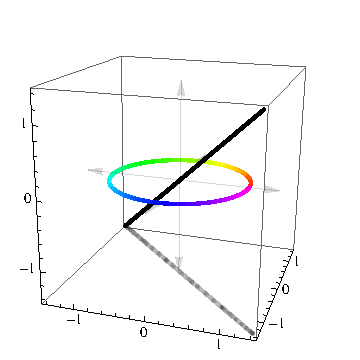
\includegraphics[ width = 2.5in ]{pdf/post_mortemII/3_2_1_a} &
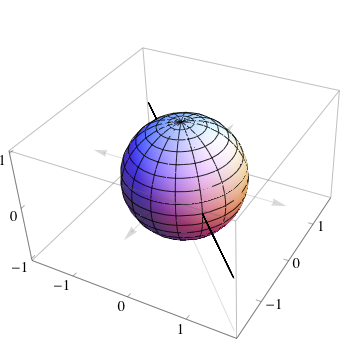
\includegraphics[ width = 2.5in ]{pdf/post_mortemII/3_2_1_t_a} \\
%%
vector space mappings & vector space mappings\\
(Domain) $\real{2} \mapsto \real{3}$ (Codomain) & (Codomain) $\real{3} \mapsto \real{2}$ (Domain)\\
 $\textellipsis$ & $\textellipsis$ \\
 matrix image & transpose matrix image \\
unit circle $\mapsto$ line & unit sphere $\mapsto$ line\\
 $\textellipsis$ & $\textellipsis$ \\
column rank deficient & row rank deficient\\
frustrated map & frustrated map\\
 $\textellipsis$ & $\textellipsis$ \\
 $\nexists\ \AinvL$ &  $\nexists\ \AinvR$ \\[10pt]
\end{tabular}
\end{center}
\label{tab:interpII:c}
\caption{Frustration in both directions, domain to codomain and back. The matrix rank is less than the number of rows $(\rho<m)$ and less than the number of columns $(\rho<n)$. The line is shown in black because the mapping is not one-to-one; multiple points in the target map to the same point in the image. Both figures show a projection of the image onto the floor of the figure. Because the matrix is both column and rank deficient there is neither a left nor a right inverse.}
\end{table}

\endinput
